\mysection{Introduction}
\label{section:introduction}

Over the last few years, we have witnessed an increase in the number and
diversity of personal computing devices. These include smart phones, tablets,
smart glasses, watches, and a variety of special-purpose embedded devices, such
as health monitors and sensors. We can expect these devices to become integral
parts of end-users' daily lives, \eg~smart glasses used for prescription vision
correction, and watches used as continuous health monitors. As a result of
these developments, smart devices will come to be used in a wide variety of
settings, such as the home, in social settings, and at school and work.
End-users will carry these devices as they go, and expect them to connect and
work with the environments at the places they visit.

% With the ubiquitous use of smart devices, we as a society need to address the
% use of these devices in \textit{restricted spaces}. We define such spaces to
% be environments that impose specific policies (often unwritten) on the use of
% smart devices. Examples of restricted spaces abound in today's society, and
% the policies that they impose vary widely. 
%
As smart devices evolve, their computing power will continue to increase and so
will the quality and diversity of periperhals available on them. While this is
generally a desirable trend, there are environments in which highly-capable
smart devices may be misused to gather and exfiltrate information from the
environment, or smuggle unauthorized information into the environment. This may
happen either through overt malice by the device owner, or unintentionally, via
malicious apps accidentially installed on the device. Examples of such
environments abound in today's society, and they impose a wide variety of
policies (often unwritten) governing the use of smart devices. Enterprises
typically forbid employees' personal devices from connecting to corporate
networks or storing corporate data. Federal institutions and laboratories that
process sensitive information place even more stringent restrictions, often
requiring employees and visitors to place personal devices in Faraday cages
before entering certain areas. In the classroom setting, students are often
forbidden from using the aid of smart devices during examinations. Even outside
work and school, there may be privacy concerns that restrict how smart devices
are used. For example, certain restaurants and bars ban patrons from wearing
smart glasses~\cite{url:glassban}. In social settings, people may be
uncomfortable at the thought of their conversations being recorded by smart
devices.  We use the term \textit{restricted spaces} to refer to such
environments.

The mechanisms traditionally used to regulate device use in restricted spaces
are \adhoc.  Consider, for instance, the restricted spaces discussed above. In
the enterprise setting, employees are given a separate work laptop/phone that
can connect to the corporate network. They are also implicitly, or by contract,
forbidden from copying data from these corporate devices onto their personal
devices. In the federal setting, employees and visitors must undergo physical
security checks to ensure that they are not carrying electronic equipment,
while in the classroom setting, proctors enforce compliance. And in social
settings, enforcement is informal and left to privacy-conscious patrons or
hosts.

Going forward, such \adhoc\ methods will prove inadequate. First, our
increasing reliance on smart devices will make traditional methods difficult to
use. For example, it would not be possible to ask an employee or a student with
prescription smart glasses to refrain from using the device. In this case, the
right solution would be to allow the smart glass to be used as a vision
corrector but regulate the use of its camera, microphone or WiFi interfaces.
Second, the increasing diversity of smart devices will make it hard to identify
policy violations (even if the devices are not used covertly). For example,
there is already evidence that students cheat on exams by connecting to the
Internet using smart phones~\cite{url:examcheating}. Recent research has
demonstrated even subtler methods to outsmart proctors via the use of smart
watches~\cite{smartwatch:fc14}. And third, in enterprise settings, current
trends indicate that employees may be encouraged to use their personal devices
for corporate purposes. This \textit{bring your own device} (BYOD) trend has
numerous benefits, such as device consolidation and reducing the enterprise's
cost of device procurement. With BYOD, it is imperative to ensure that employee
devices adhere to corporate policies within the enterprise.

Given these reasons, we posit that a systematic method is needed to ensure that
personal devices comply with the policies of the restricted spaces within which
they are used. Such a method would benefit both the \textit{hosts} who own or
control the restricted space and the \textit{guests} who use the smart device.
Hosts will have greater assurance that smart devices used in their spaces
conform to their policies. On the other hand, guests can benefit from and be
more open about their use of smart devices in the host's restricted space.

\begin{figure*}[t!]
\setcaptionrule
\centering
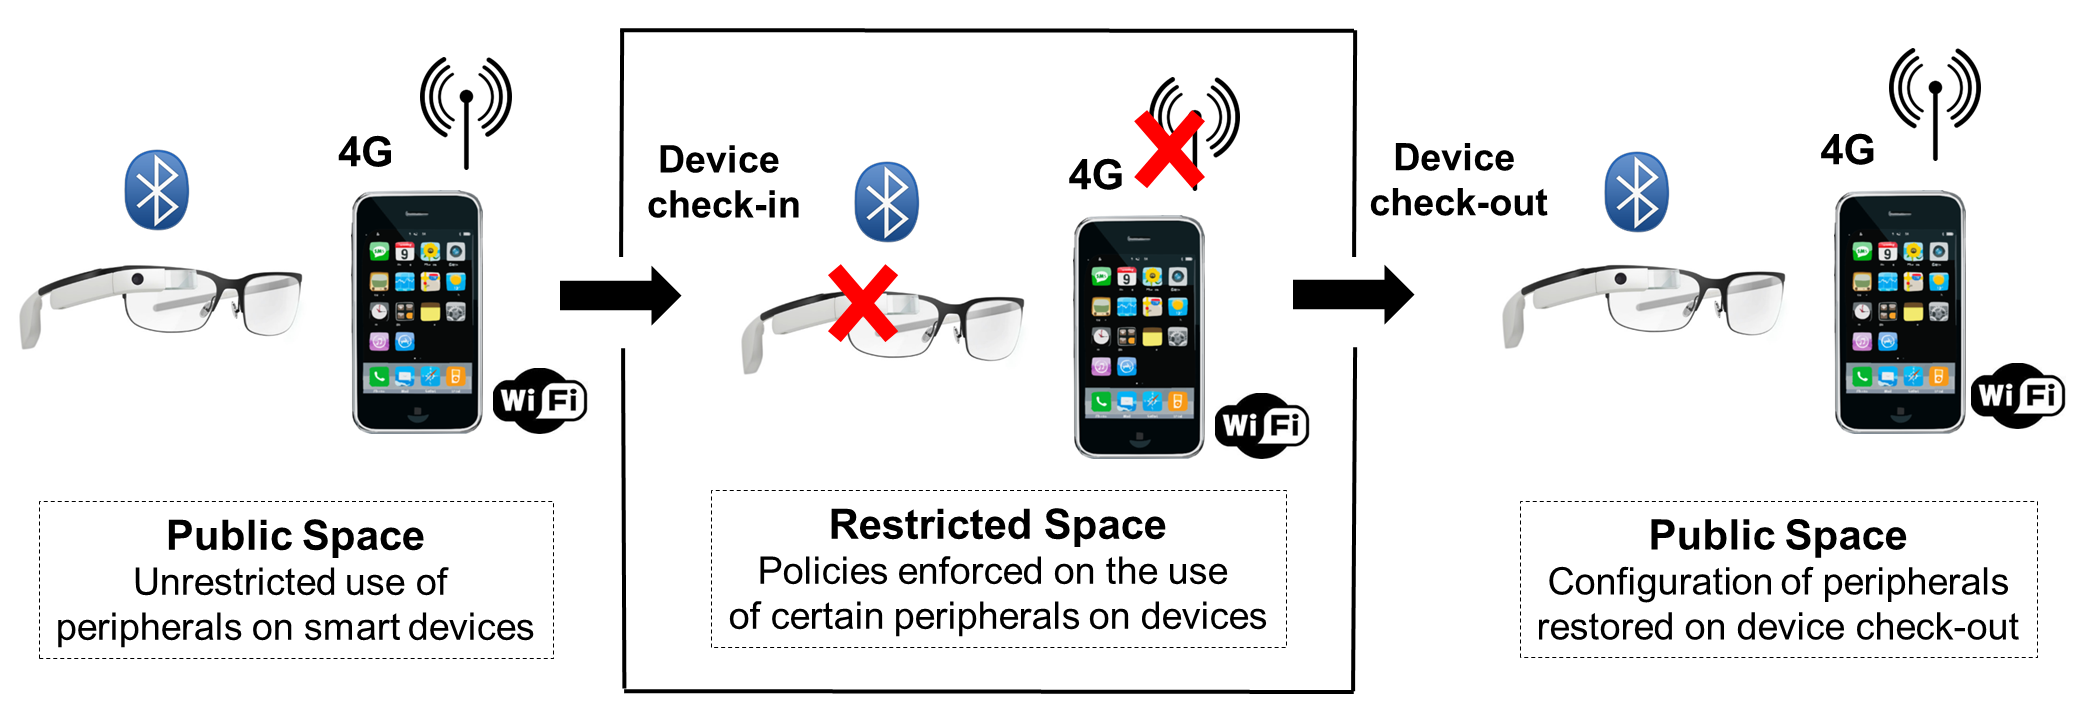
\includegraphics[keepaspectratio=true,width=0.85\textwidth]{figures/restricted-space.png}
%\indent\vspace{-0.5cm}
\mycaption{An overview of our restricted space model. Guests ``check-in''
devices when entering restricted spaces. During check-in, hosts inspect,
analyze and modify the configurations of these devices in accordance with their
usage policies. In this example, the host restricts the use of the camera on
the smart glass, and the 4G data interface on the smart phone. However, the
glass can continue to use its Bluetooth interface to pair with the smart phone,
while the phone can use WiFi.  When guests leave the restricted space, they
``check-out'' their devices, which the host then restores to their original
configurations.}
{\label{figure:restrictedspaces}}
%\indent\vspace{-0.55cm}
\end{figure*}


In this paper, we present an approach for hosts to remotely regulate the use of
smart guest devices in restricted spaces. Our approach recognizes that policies
to govern device use vary widely across restricted spaces, and therefore
cleanly separates policy from mechanism. Policies are specified by hosts and
could, for instance, require guests to prove that their devices are free of
certain forms or malicious software, or restrict the use of certain peripherals
on the devices, \eg\ camera, WiFi, 3G/4G. 
% In \sectref{section:policy}, we present a number of scenarios where
% controlling peripherals would be useful.

The enforcement mechanism itself is implemented on the guests' device(s) and
simply enforces the host's policies. This mechanism must have three key
properties.  First, it must be \textit{trusted} by both hosts and guests, and
is therefore part of the trusted computing base (TCB). Hosts trust the
mechanism to correctly enforce policies on guest devices. On the other hand,
guests trust the mechanism to authenticate hosts. Host authentication is
important because malicious or untrusted hosts could otherwise abuse the
mechanism to compromise guest security and privacy.  Second, the mechanism must
have the ability to \textit{inspect} guest devices and \textit{make
configuration changes} to enforce hosts' policies.  And third, the mechanism
must be \textit{minimal}, and not bloat the size of the TCB executing on guest
devices.

We describe an approach to implement this enforcement mechanism using
\textit{remote memory operations} on the guest device. Hosts use these
operations to remotely inspect and modify the memory contents of the guest
device based on its policies. The host must be able to ensure that these
operations are performed correctly on the guest device. Thus, we cannot rely on
the guest's operating system to enforce these operations because it may be
malicious (or compromised by malware). We therefore rely on \textit{trusted
hardware} in the guest's device to provide a root of trust, which provides the
host with the desired assurances.  In particular, our prototype uses the ARM
TrustZone architecture~\cite{armtz} as the root of trust. Devices that use the
ARM TrustZone are now commercially available and widely
deployed~\cite{knox:ccs14}. We rely on the ARM TrustZone to bootstrap trust in
our mechanism's TCB, which executes on the guest. 

The use of trusted hardware enables our approach to offer an attractive
feature---using the ARM TrustZone, a guest device can prove to the host (using
\textit{verification tokens}, introduced in \sectref{section:mechanism:tokens})
that it was policy compliant for the duration of its stay in the restricted
space. Malicious guest devices, which may have violated the host's policies in
the restricted space, will not be able to provide such a proof, and can
therefore be apprehended by the host. The ability to handle malicious guest
devices is a significant difference from prior projects with related
goals~\cite{worlddriven:ccs14,blindspot:2009,markit:upside14}, which have
assumed that the guest devices are benign and will not attempt to bypass the
host's policies within the restricted space.

To summarize, the main contributions of this paper are the following:
%
\begin{mybullet}
%
\item \textit{Restricted space model.} We introduce the restricted space model
for smart personal devices (\sectref{section:usagemodel}). This model is of
independent interest due to the growing number of environments that restrict
smart device use. We also present multiple examples of policies that may be
enforced in restricted spaces (\sectref{section:policy}).
%
\item \textit{Enforcement mechanism.} We present the design of a mechanism for
hosts to enforce policies on guest device use (\sectref{section:mechanism}).
Our mechanism allows hosts to remotely inspect and control a guest device using
a simple interface with two operations: remote memory reads, and remote memory
writes. The mechanism allows hosts to request a proof from guest devices that
they are policy compliant; only compliant devices can provide a proof that will
be acceptable to the hosts. Finally, the mechanism ensures that only
authenticated hosts can control guest devices, and provides a vetting service
that allows guests to check the safety of the host's requests
(\sectref{section:vetting}). 
%
\item \textit{Prototype implementation.} We demonstrate a prototype
implementation of the mechanism using the ARM TrustZone hardware as a root of
trust on guest devices. Our design/implementation is minimal, thereby ensuring
a small TCB on guest devices (\sectref{section:evaluation}).
%
\end{mybullet}
